\documentclass[a4paper,12pt]{article}

% packages
\usepackage[T1]{fontenc}
\usepackage[latin1]{inputenc}
\usepackage{amsmath}
\usepackage{amsfonts}
\usepackage{amssymb}
\usepackage{graphicx}
\usepackage{listings}
\usepackage{url}
\usepackage[usenames]{xcolor}
\usepackage[top=3cm, bottom=3cm, left=3cm, right=3cm]{geometry}

% Path to the pictures
\graphicspath{ {images/} }

% Customized style to display c++ source code
\lstdefinestyle{customcpp}{
  backgroundcolor=\color{gray!15},
  belowcaptionskip=1\baselineskip,
  breaklines=true,
  frame=L,
  xleftmargin=\parindent,
  language=C++,
  showstringspaces=false,
  basicstyle=\footnotesize\ttfamily,
  keywordstyle=\bfseries\color{green!40!black},
  commentstyle=\itshape\color{purple!40!black},
  identifierstyle=\color{blue},
  stringstyle=\color{orange},
}
\lstset{style=customcpp}

% Title page definition

\makeatletter
\def\maketitle{%
  \null
  \thispagestyle{empty}%
  \begin{center}\leavevmode
    \normalfont
    {}
    \vskip 1.3cm
    {\Huge \@title\par}%
    \vskip 0.3cm
    {\Large Version: 0.8.0\par}%
    \vskip 0.3cm
    {\Large \@author\par}%
    \vskip 2cm
    {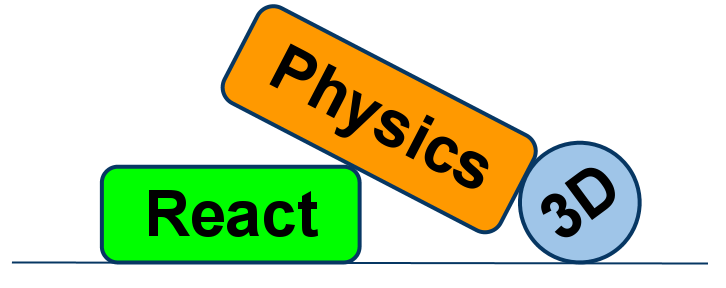
\includegraphics[height=5cm]{images/ReactPhysics3DLogo.png}}
    \vskip 2cm
    {\large{\url{http://www.reactphysics3d.com}}}
    \vskip 0.2cm
   {\large \@date}%
  \end{center}%
  \vfill
  \null
  \cleardoublepage
  }
\makeatother


\begin{document}
   \author{Daniel Chappuis}
   \title{ReactPhysics3D library \\ User Manual}
   \maketitle

   \tableofcontents

   \newpage


   \section{Introduction}

  ReactPhysics3D is an open source C++ physics engine library that can be used
  in 3D simulations and games. The library is released under the ZLib license.

   \section{Features}

   The ReactPhysics3D library has the following features:

   \begin{itemize}
    \item Rigid body dynamics
    \item Discrete collision detection
    \item Collision shapes (Sphere, Box, Cone, Cylinder, Capsule, Convex Mesh, Static Concave Mesh, Height Field)
    \item Multiple collision shapes per body
    \item Broadphase collision detection (Dynamic AABB tree)
    \item Narrowphase collision detection (GJK/EPA)
    \item Collision response and friction (Sequential Impulses Solver)
    \item Joints (Ball and Socket, Hinge, Slider, Fixed)
    \item Collision filtering with categories
    \item Ray casting
    \item Sleeping technique for inactive bodies
    \item Integrated Profiler
    \item Multi-platform (Windows, Linux, Mac OS X)
    \item Documentation (User manual and Doxygen API)
    \item Testbed application with demos
    \item Unit tests
   \end{itemize}

    \section{License}

    The ReactPhysics3D library is released under the open-source ZLib license. For more information, read the "LICENSE" file.

    \section{Building the library}
    \label{sec:building}

    You should use the CMake software to generate the makefiles or the
    project files for your IDE. CMake can be downloaded at
    \url{http://www.cmake.org} or using your package-management program
    (apt, yum, \dots) on Linux. Then, you will be able to compile the library to create the static library
    file. In order to use ReactPhysics3D in your application, you can link your program with this static library.
    If you have never used cmake before, you should read the page \url{http://www.cmake.org/cmake/help/runningcmake.html} as
    it contains a lot of useful information. \\

    It is also possible to compile the testbed application using CMake. The testbed application contains different
    demo scenes using the ReactPhysics3D library.
xs
    \subsection{CMake using the command line (Linux and Mac OS X)}

    Now, we will see how to build the ReactPhysics3D library using the CMake tool with the command line.
    First, create a folder where you want to build the library. Then go into that folder and run
    the \texttt{ccmake} command: \\

    \texttt{ccmake \textless path\_to\_library\_source\textgreater} \\

    \begin{sloppypar}
    where \texttt{\textless path\_to\_library\_source\textgreater} must be replaced
    by the path to the \texttt{reactphysics3d-0.6.0/} folder. It is the folder that
    contains the \texttt{CMakeLists.txt} file. Running this command will launch the CMake command line interface.
    Hit the 'c' key to configure the project. There, you can also change some predefined variables (see section \ref{sec:cmakevariables} for more details)
    and then, hit the 'c' key again. Once you have set all the values as you like, you can hit the 'g' key to generate the makefiles in the build directory
    that you have created before and exit. \\

    Now that you have generated the makefiles with the CMake software, you can compile the code to build the static library in the
    \texttt{/lib} folder with the following command in your build directory: \\

    \end{sloppypar}

    \texttt{make}

    \subsection{CMake using the graphical interface (Linux, Mac OS X and Windows)}

     You can also use the graphical user interface of CMake. To do this,
     run the \texttt{cmake-gui} program. The program will ask you for the
     source folder which is the \texttt{reactphysics3d-0.6.0/} folder of
     the library. You will also have to select a folder where you want to
     build the library and the testbed application. Select any empty folder that
     is on your system. Then, you can click on \texttt{Configure}. CMake will ask you to choose an IDE that is on
     your system. For instance, you can select Visual Studio, Qt Creator, XCode, ... Then, you
     can change the compilation options. See section \ref{sec:cmakevariables} to see what are the possible options.
     Once this is done, you can click on \texttt{Configure} again and finally on \texttt{Generate}. \\

     Now, if you go into the folder you have chosen to build the
     library, you should be able to open the project file that corresponds to your IDE and compile
     the library. \\

     \subsection{CMake Variables}
     \label{sec:cmakevariables}

     You can find bellow the different CMake variables that you can set before generating the makefiles:

       \begin{description}
         \item[CMAKE\_BUILD\_TYPE] If this variable is set to \texttt{Debug}, the library will be compiled in debugging mode.
                                                    This mode should be used during development stage to know where things might crash.
                                                    In debugging mode, the library might run a bit slow due to all the debugging information.
                                                    However, if this variable is set to \texttt{Release}, no debugging information is stored
                                                    and therefore, it will run much faster. This mode must be used when you compile the final
                                                    release of you application.

         \item[COMPILE\_TESTBED] If this variable is \texttt{ON}, the tesbed application of the library will be compiled.
                                                         The testbed application uses OpenGL for rendering.
                                                         Take a look at the section \ref{sec:testbed} for more information about the testbed application.

         \item[COMPILE\_TESTS] If this variable is \texttt{ON}, the unit tests of the library will be compiled. You will then
                                             be able to launch the tests to make sure that they are running fine on your system.

          \item[PROFILING\_ENABLED] If this variable is \texttt{ON}, the integrated profiler will collect data while the application is running
                                                      and the profiling report will be displayed in the console at the end of the application (in the
                                                      destructor of the \texttt{DynamicsWorld} class). This might be useful to see what part of the reactphysics3d
                                                      library takes time during its execution. This variable must be set to \texttt{OFF} when you compile
                                                      the final release of your application.

          \item[DOUBLE\_PRECISION\_ENABLED] If this variable is \texttt{ON}, the library will be compiled with double floating point precision.
                                                                    Otherwise, the library will be compiled with single precision.
       \end{description}


    \section{Using ReactPhysics3D in your application}

    In order to use the library in your own application, first build
    the static library of ReactPhysics3d as described above to get the
    static library file in the \texttt{lib/} folder. Then, in your code, you have to include
    the ReactPhysics3D header file with the line: \\

    \begin{lstlisting}
// Include the ReactPhysics3D header file
#include "reactphysics3d.h"
  \end{lstlisting}

    \vspace{0.6cm}

    Note that the \texttt{reactphysics3d.h} header file can be found in the
    \texttt{src/} folder of the library. Do not forget to add the
    \texttt{src/} folder in your include directories in order that the
    \texttt{reactphysics3d.h} file is accessible in your code. \\

    Do not forget to also link your application with the ReactPhysics3D
    static library.  \\

    Then, you should be able to compile your application using the
    ReactPhysics3D library. \\

    All the classes of the library are available in the \texttt{reactphysics3d} namespace or its shorter alias
    \texttt{rp3d}. Therefore, you need to include this namespace into your code with the following declaration: \\

    \begin{lstlisting}
// Use the ReactPhysics3D namespace
using namespace reactphysics3d;
    \end{lstlisting}

    \vspace{0.6cm}

    You can also take a look at the examples and the API documentation to get a better idea of how to use the
    ReactPhysics3D library.

   \section{The Collision World}

    There are two main ways to use ReactPhysics3D. The first one is to create bodies that you have to manually move so that you can test collision between them. To do this,
    you need to create a Collision World with several Collision Bodies in it. The second way is to create bodies and let ReactPhysics3D simulate their motions automatically using the
    physics. This is done by creating Rigid Bodies in a Dynamics World instead. In summary, a Collision World is used to simply test collision between bodies that you have to manually move
    and a Dynamics World is used to create bodies that will be automatically moved using collisions, joints and forces. \\

    The \texttt{CollisionWorld} class represents a Collision World in the ReactPhysics3D library.

    \subsection{Creating the Collision World}

    If you only have to test collision between bodies, the first thing to do is to create an instance of the \texttt{CollisionWorld} class. \\

    Here is how to create a Collision World: \\

    \begin{lstlisting}

// Create the collision world
rp3d::CollisionWorld world;
    \end{lstlisting}

    \subsection{Destroying the Collision World}

    Do not forget to destroy the \texttt{CollisionWorld} instance at the end of your program in order to release the allocated memory. If the object has been created
    statically, it will be destroyed automatically at the end of the scope in which it has been created. If the object has been created dynamically (using the \texttt{new}
    operator), you need to destroy it with the \texttt{delete} operator. \\

    When the \texttt{CollisionWorld} is destroyed, all the bodies that have been added into it and that have not been destroyed already will be destroyed.
    Therefore, the pointers to the bodies of the world will become invalid after the existence of their \texttt{CollisionWorld}.

    \section{Collision Bodies}

    Once the Collision World has been created, you can create Collision Bodies into the world. A Collision Body represents an object in the Collision World.
    It has a position, an orientation and one or more collision shapes. It has to be moved manually in the Collision World. You can then
    test collisions between the Collision Bodies of the world. In ReactPhysics3D, the \texttt{CollisionBody} class is used to describe a Collision Body. \\

    If you do not want to simply test collision between your bodies but want them to move automatically according to the physics, you should use Rigid Bodies in a
    Dynamics World instead. See section \ref{sec:dynamicsworld} for more information about the Dynamics World and section \ref{sec:rigidbody} if you would like to know more
    about the Rigid Bodies.

    \subsection{Creating a Collision Body}

    In order to create a Collision Body, you need to specify its transform. The transform describes the initial
    position and orientation of the body in the world. You need to create an instance of the \texttt{Transform} class with a vector describing the
    initial position and a quaternion for the initial orientation of the body. \\

    In order to test collision between your body and other bodies in the world, you need to add one or several collision shapes to your body.
    Take a look at section \ref{sec:collisionshapes} to learn about the different collision shapes and how to create them. \\

    You need to call the \texttt{CollisionWorld::createCollisionBody()} method to create a Collision Body in the world previously created. This method will return a pointer to the instance
    of the \texttt{CollisionBody} class that has been created internally. You will then be able to use that pointer to get or set values of the body. \\

    You can see in the following code how to create a Collision Body in the world. \\

    \begin{lstlisting}

// Initial position and orientation of the collision body
rp3d::Vector3 initPosition(0.0, 3.0, 0.0);
rp3d::Quaternion initOrientation = rp3d::Quaternion::identity();
rp3d::Transform transform(initPosition, initOrientation);

// Create a collision body in the world
rp3d::CollisionBody* body;
body = world.createCollisionBody(transform);
  \end{lstlisting}

    \subsection{Moving a Collision Body}

    A Collision Body has to be moved manually in the world. To do that, you need to use the \texttt{CollisionBody::setTransform()} method to set a new position and new
   orientation to the body.

     \begin{lstlisting}

// New position and orientation of the collision body
rp3d::Vector3 position(10.0, 3.0, 0.0);
rp3d::Quaternion orientation = rp3d::Quaternion::identity();
rp3d::Transform newTransform(position, orientation);

// Move the collision body
body->setTransform(newTransform);
  \end{lstlisting}

    \subsection{Destroying a Collision Body}

    \begin{sloppypar}
    In order to destroy a Collision Body from the world, you need to use the \texttt{CollisionWorld::destroyCollisionBody()} method. You need to use the pointer to the body you
    want to destroy in argument. Note that after calling that method, the pointer will not be valid anymore and therefore, you should not use it. \\
    \end{sloppypar}

    Here is how to destroy a Collision Body: \\

    \begin{lstlisting}
// Here, world is an instance of the CollisionWorld class
// and body is a CollisionBody* pointer

// Destroy the collision body and remove it from the world
world.destroyCollisionBody(body);
  \end{lstlisting}

    \section{The Dynamics World}
    \label{sec:dynamicsworld}

    The Collision World of the previous section is used to manually move the bodies and check for collision between them. On the other side, the Dynamics World
    is used to automatically simulate the motion of your bodies using the physics. You do not have to move the bodies manually (but you still can if needed).
    The Dynamics World will contain the bodies and joints that you create. You will then be able to run your simulation across time by updating the world at each frame.
    The \texttt{DynamicsWorld} class (which inherits from the \texttt{CollisionWorld} class) represents a Dynamics World in the ReactPhysics3D library.

    \subsection{Creating the Dynamics World}

    The first thing you have to do when you want to simulate the dynamics of rigid bodies in time is to create an instance
    of the \texttt{DynamicsWorld}. You need to specify the gravity acceleration vector (in $m / s^2$) in the world as parameter. Note that gravity is
    activated by default when you create the world. \\

    Here is how to create the Dynamics World: \\

    \begin{lstlisting}
// Gravity vector
rp3d::Vector3 gravity(0.0, -9.81, 0.0);

// Create the dynamics world
rp3d::DynamicsWorld world(gravity);
  \end{lstlisting}

    \subsection{Customizing the Dynamics World}

    \subsubsection{Solver parameters}

    ReactPhysics3D uses an iterative solver to compute the contacts and joints. For contacts, there is a unique velocity solver and for joints there are a velocity and a
    position solver. By default, the number of iterations of the velocity solver is 10 and the number of iterations for the position solver is 5. It is possible to
    change the number of iterations for both solvers. \\

    To do this, you need to use the following two methods: \\

    \begin{lstlisting}
// Change the number of iterations of the velocity solver
world.setNbIterationsVelocitySolver(15);

// Change the number of iterations of the position solver
world.setNbIterationsPositionSolver(8);
  \end{lstlisting}

    \vspace{0.6cm}

    Increasing the number of iterations of the solvers will make the simulation more precise but also more expensive to compute. Therefore, you need to change
    those values only if needed.

    \subsubsection{Sleeping}
    \label{sec:sleeping}

    The purpose of the sleeping technique is to deactivate resting bodies so that they are not simulated anymore. This is used to save computation time because simulating
    many bodies is costly.
    A sleeping body (or group of sleeping bodies) is awaken as soon as another body collides with it or a joint in which it is involed is enabled. The sleeping technique
    is enabled by default. You can disable it using the following method: \\

    \begin{lstlisting}
// Disable the sleeping technique
world.enableSleeping(false);
  \end{lstlisting}

    \vspace{0.6cm}

    Note that it is not recommended to disable the sleeping technique because the simulation might become slower. It is also possible to deactivate the sleeping technique on a
    per body basis. See section \ref{sec:rigidbodysleeping} for more information. \\

    \begin{sloppypar}
      A body is put to sleep when its linear and angular velocity stay under a given velocity threshold for a certain amount of time (one second by default). It is possible to
      change the two
      linear and angular velocity thresholds using the two methods \texttt{DynamicsWorld::setSleepLinearVelocity()} and \texttt{DynamicsWorld::setSleepAngularVelocity()}.
      Note that the velocities must
      be specified in meters per second. You can also change the amount of time (in seconds) the velocity of a body needs to stay under the threshold to be considered
      sleeping. To do this, use the
    \texttt{DynamicsWorld::setTimeBeforeSleep()} method.
   \end{sloppypar}

    \subsection{Updating the Dynamics World}
    \label{sec:updating_dynamics_world}

    The \texttt{DynamicsWorld} is used to simulate physics through time. It has to be updated each time you want to simulate a step forward in time. Most of the time,
    you want to update the world right before rendering a new frame in a real-time application. \\

    To update the physics world, you need to use the \texttt{DynamicsWorld::update()} method. This method will perform collision detection and update the
    position and orientation of the bodies and joints. After updating the world, you will be able to get the new position and orientation of your bodies for the next
    frame to render. This method requires a \emph{timeStep} parameter. This is the amount of time you want to advance the physics simulation (in seconds). \\

    The smaller the time step you pick, the more precise the simulation will be but it can also be more expensive to compute. For a real-time application, you
    probably want a time step of at most $\frac{1}{60}$ seconds to
    have at least a 60 Hz framerate. Most of the time, physics engines prefer to work with a constant time step. It means that you should always call
    the \texttt{DynamicsWorld::update()} method with the same time step parameter. You do not want to use the time between two frames as your time step because it will
    not be constant. \\

    You can use the following technique. First, you choose a constant time step for the physics. Let say the time step is $\frac{1}{60}$ seconds. Then, at each frame,
    you compute the time difference between the current frame and the previous one and you accumulate this difference in a variable called \emph{accumulator}. The accumulator
    is initialized to zero at the beginning of your application and is updated at each frame. The idea is to divide the time in the accumulator in several constant time steps.
    For instance, if your accumulator contains $0.145$ seconds, it means that we can take $8$ physics steps of $\frac{1}{60}$ seconds during the current frame. Note that
    $0.012$ seconds will remain in the accumulator and will probably be used in the next frame. As you can see, multiple physics steps can be taken at each frame. It is
    important to understand that each call to the \texttt{DynamicsWorld::update()} method is done using a constant time step that is not varying with the framerate. \\

    Here is what the code looks like at each frame: \\

    \begin{lstlisting}

// Constant physics time step
const float timeStep = 1.0 / 60.0;

// Get the current system time
long double currentFrameTime = getCurrentSystemTime();

// Compute the time difference between the two frames
long double deltaTime  = currentFrameTime - previousFrameTime;

// Update the previous time
previousFrameTime = currentFrameTime;

// Add the time difference in the accumulator
accumulator += mDeltaTime;

// While there is enough accumulated time to take
// one or several physics steps
while (accumulator >= timeStep) {

    // Update the Dynamics world with a constant time step
    dynamicsWorld->update(timeStep);

    // Decrease the accumulated time
    accumulator -= timeStep;
}

    \end{lstlisting}


    \subsection{Destroying the Dynamics World}

    Do not forget to destroy the \texttt{DynamicsWorld} instance at the end of your program in order to release the allocated memory. If the object has been created
    statically, it will automatically be destroyed at the end of the scope in which it has been created. If the object has been created dynamically (using the
    \texttt{new} operator), you need to destroy it with the \texttt{delete} operator. \\

    When the \texttt{DynamicsWorld} is destroyed, all the bodies and joints that have been added into it and that have not been destroyed already will be destroyed.
    Therefore, the pointers to the bodies and joints of the world will become invalid after the existence of their \texttt{DynamicsWorld}.

    \section{Rigid Bodies}
    \label{sec:rigidbody}

    Once the Dynamics World has been created, you can create rigid bodies into the world. A Rigid Body represents an object that you want to simulate in the world.
    It has a mass, a position, an orientation and one or several collision shapes. The Dynamics World will compute collisions between the bodies and will update their position
    and orientation accordingly at each time step. You can also create joints between the bodies in the world. In ReactPhysics3D, the \texttt{RigidBody} class
    (which inherits from the \texttt{CollisionBody} class) is used to describe a Rigid Body.

    \subsection{Creating a Rigid Body}

    In order to create a Rigid Body, you need to specify its transform. The transform describes the initial
    position and orientation of the body in the world. You need to create an instance of the \texttt{Transform} class with a vector describing the
    initial position and a quaternion for the initial orientation of the body. \\

    You need to call the \texttt{DynamicsWorld::createRigidBody()} method to create a Rigid Body in the world previously created. This method will return a pointer to the
    instance of the \texttt{RigidBody} object that has been created internally. You will then be able to use that pointer to get or set values of the body. \\

    You can see in the following code how to create a Rigid Body in your world: \\

    \begin{lstlisting}
// Initial position and orientation of the rigid body
rp3d::Vector3 initPosition(0.0, 3.0, 0.0);
rp3d::Quaternion initOrientation = rp3d::Quaternion::identity();
rp3d::Transform transform(initPosition, initOrientation);

// Create a rigid body in the world
rp3d::RigidBody* body;
body = dynamicsWorld.createRigidBody(transform);
    \end{lstlisting}

    \vspace{0.6cm}

    Once your Rigid Body has been created in the world, you need to add one or several collision shapes to it. Take a look at section \ref{sec:collisionshapes} to learn
    about the different collision shapes and how to create them. \\

    \subsection{Customizing a Rigid Body}

    Once a Rigid Body has been created, you can change some of its properties.

    \subsubsection{Type of a Rigid Body (static, kinematic or dynamic)}

    \begin{sloppypar}
        There are three types of bodies: \emph{static}, \emph{kinematic} and \emph{dynamic}. A \emph{static} body has infinite mass, zero velocity but its position can be
        changed manually. Moreover, a static body does not collide with other static or kinematic bodies. On the other side, a \emph{kinematic} body has infinite mass, its velocity can be
        changed manually and its position is computed by the physics engine. A kinematic body does not collide with other static or kinematic bodies. Finally, A \emph{dynamic} body
        has non-zero mass, non-zero velocity determined by forces and its position is determined by the physics engine. Moreover, a dynamic body can collide with other dynamic, static or
        kinematic bodies. \\
    \end{sloppypar}

    When you create a new body in the world, it is of dynamic type by default. You can change the type of the body using the \texttt{CollisionBody::setType()}
    method as follows:\\

    \begin{lstlisting}
// Change the type of the body to Kinematic
body->setType(KINEMATIC);
  \end{lstlisting}

    \subsubsection{Gravity}

    By default, all the rigid bodies with react to the gravity force of the world. If you do not want the gravity to be applied to a given body, you can disable
    it using the \texttt{RigidBody::enableGravity()} method as in the following example : \\

    \begin{lstlisting}
// Disable gravity for this body
rigidBody->enableGravity(false);
  \end{lstlisting}

    \subsubsection{Material of a Rigid Body}

    The material of a rigid body is used to describe the physical properties it is made of. The \texttt{Material} class represents the material of a body. Each body that
    you create will have a default material. You can get the material of the rigid body using the \texttt{RigidBody::getMaterial()} method. Then, you will be able to change some
    properties. \\

    For instance, you can change the bounciness of the rigid body. The bounciness is a value between 0 and 1. The value 1 is used for a very bouncy object and the value 0 means that
    the body will not be bouncy at all. To change the bounciness of the material, you can use the \texttt{Material::setBounciness()} method. \\

    You are also able to change the friction coefficient of the body. This value needs to be between 0 and 1. If the value is 0, no friction will be applied when the body is in contact with
    another body. However, if the value is 1, the friction force will be high. You can change the friction coefficient of the material with the
    \texttt{Material::setFrictionCoefficient()} method. \\

    You can use the material to add rolling resistance to a rigid body. Rolling resistance can be used to stop
    a rolling object on a flat surface for instance. You should use this only with SphereShape,
    CapsuleShape, CylinderShape or ConeShape collision shapes. By default, rolling resistance is zero but you can
    set a positive value using the \texttt{Material::setRollingResistance()} method to increase resistance. \\

    Here is how to get the material of a rigid body and how to modify some of its properties : \\

    \begin{lstlisting}
// Get the current material of the body
rp3d::Material& material = rigidBody->getMaterial();

// Change the bounciness of the body
material.setBounciness(rp3d::decimal(0.4));

// Change the friction coefficient of the body
material.setFrictionCoefficient(rp3d::decimal(0.2));
  \end{lstlisting}

    \subsubsection{Velocity Damping}

    \begin{sloppypar}
      Damping is the effect of reducing the velocity of the rigid body during the simulation to simulate effects like air friction for instance. By default, no damping
      is applied. However, you can choose to damp the linear or/and the angular velocity of a rigid body. For instance, without angular damping a pendulum will never come
      to rest. You need to use the \texttt{RigidBody::setLinearDamping()} and \texttt{RigidBody::setAngularDamping()} methods to change the damping values. The damping
      value has to be positive and a value of zero means no damping at all.
    \end{sloppypar}

    \subsubsection{Sleeping}
    \label{sec:rigidbodysleeping}

    As described in section \ref{sec:sleeping}, the sleeping technique is used to disable the simulation of resting bodies. By default, the bodies are allowed to sleep
    when they come to rest. However, if you do not want a given body to be put to sleep, you can use the \texttt{Body::setIsAllowedToSleep()} method as in the next example : \\

   \begin{lstlisting}
// This rigid body cannot sleep
rigidBody->setIsAllowedToSleep(false);
 \end{lstlisting}

    \subsubsection{Applying Force or Torque to a Rigid Body}

    During the simulation, you can apply a force or a torque to a given rigid body. First, you can apply a force to the center of mass of the rigid body using the
    \texttt{RigidBody::applyForceToCenter()} method. You need to specify the force vector (in Newton) as a parameter. If the force is applied to the center of mass, no
    torque will be created and only the linear motion of the body will be affected. \\

    \begin{lstlisting}
// Force vector (in Newton)
rp3d::Vector3 force(2.0, 0.0, 0.0);

// Apply a force to the center of the body
rigidBody->applyForceToCenter(force);
  \end{lstlisting}

    \vspace{0.6cm}

    \begin{sloppypar}
        You can also apply a force to any given point (in world-space) using the \texttt{RigidBody::applyForce()} method. You need to specify the force vector (in Newton) and the point
        (in world-space) where to apply the given force. Note that if the point is not the center of mass of the body, applying a force will generate some torque and therefore, the
        angular motion of the body will be affected as well. \\
    \end{sloppypar}

    \begin{lstlisting}
// Force vector (in Newton)
rp3d::Vector3 force(2.0, 0.0, 0.0);

// Point where the force is applied
rp3d::Vector3 point(4.0, 5.0, 6.0);

// Apply a force to the body
rigidBody->applyForce(force, point);
  \end{lstlisting}

    \vspace{0.6cm}

     \begin{sloppypar}
        It is also possible to apply a torque to a given body using the \texttt{RigidBody::applyTorque()} method. You simply need to specify the torque vector (in Newton $\cdot$ meter) as
        in the following example: \\
     \end{sloppypar}

    \begin{lstlisting}
// Torque vector
rp3d::Vector3 torque(0.0, 3.0, 0.0);

// Apply a torque to the body
rigidBody->applyTorque(torque);
  \end{lstlisting}

    \vspace{0.6cm}

    Note that when you call the previous methods, the specified force/torque will be added to the total force/torque applied to the rigid body and that at the end of each call to the
    \texttt{DynamicsWorld::update()}, the total force/torque of all the rigid bodies will be reset to zero. Therefore, you need to call the previous methods during several frames
    if you want the force/torque to be applied during a certain amount of time.

    \subsection{Updating a Rigid Body}

    When you call the \texttt{DynamicsWorld::update()} method, the collisions between the bodies are computed and the joints are evaluated. Then, the bodies position
    and orientation are updated accordingly. \\

    Remember that in section \ref{sec:updating_dynamics_world} we were using a time accumulator in order to always have fixed physics time steps.
    Now imagine a situation where the rendering frame rate is higher than the the physics frame rate. It means that at the end of most rendering
    frames there will be some time left in the accumulator for the physics time that has not been simulated yet by the physics engine.
    It means that we are rendering the state of the physics simulation at a time different from the rendering time which can cause a visual stuttering effect. \\

    To solve this, the idea is to interpolate between the previous and current physics state of the simulation based on how much time is left in the
    accumulator. First we compute the interpolation factor as follows: \\

    \begin{lstlisting}

     // Compute the interpolation factor ("accumulator" is the time left in the accumulator and
     // "dt" is the physics time step)
     const float interpolationFactor = accumulator / dt;
   \end{lstlisting}

   \vspace{0.6cm}

   Then we get the current transform of the rigid body and use it with the previous transform (transform at the previous frame) to
   compute the interpolated transform as in the following code: \\

    \begin{lstlisting}

      // Get the current transform of the rigid body
      rp3d::Transform currentTransform = body->getTransform();

      // Interpolate the transform between the previous one and the new one
      rp3d::Transform interpolatedTransform = rp3d::Transform::interpolateTransforms(previousTransform, currentTransform, interpolationFactor);
    \end{lstlisting}

    \vspace{0.6cm}

    If you need the array with the corresponding $4 \times 4$ OpenGL transformation matrix, you can use the \texttt{Transform::getOpenGLMatrix()} method as in the
    following code: \\

    \begin{lstlisting}
      // Get the OpenGL matrix array of the transform
      float matrix[16];
      transform.getOpenGLMatrix(matrix);
  \end{lstlisting}

    \subsection{Destroying a Rigid Body}

    \begin{sloppypar}
    It is really simple to destroy a rigid body. You simply need to use the \texttt{DynamicsWorld::destroyRigidBody()} method. You need to use the pointer to the body you
    want to destroy as a parameter. Note that after calling that method, the pointer will not be valid anymore and therefore, you should not use it. Note that you must
    destroy all the rigid bodies at the end of the simulation before you destroy the world. When you destroy a rigid body that was part of a joint, that joint will be
    automatically destroyed as well. \\
    \end{sloppypar}

    Here is how to destroy a rigid body: \\

    \begin{lstlisting}
// Here, world is an instance of the DynamicsWorld class
// and body is a RigidBody* pointer

// Destroy the rigid body
world.destroyRigidBody(body);
  \end{lstlisting}

    \section{Collision Shapes}
    \label{sec:collisionshapes}

    Once you have created a Collision Body or a Rigid Body in the world, you need to add one or more collision shapes into it so that it is able to collide with other bodies.
    This section describes all the collision shapes available in the ReactPhysics3D library and how to use them. \\

    The Collision Shapes are also the way to represent the mass of a Rigid Body. Whenever you add a collision shape to a Rigid Body, you need to specify the mass of the shape.
    Then the Rigid Body will recompute its total mass, its center of mass and its inertia tensor taking into account all its collision shapes. Therefore, you do not have to compute
    those things by yourself. However, if needed, you can also specify your own center of mass or inertia tensor. Note that the inertia tensor is a $3 \times 3$ matrix describing
    how the mass is distributed inside the rigid body which will be used to calculate its rotation. The inertia tensor depends on the mass and the shape of the body. \\

    Every collision shapes use a \emph{collision margin} which is a small distance around the shape that is used internally in the collision detection.
    Some collision shapes have their collision margin integrated into the shape that you define and therefore you do not have to worry about it.
    However, for some collision shapes, the collision margin is added around the shape that you define and therefore, you might have to compensate
    for this small margin when you render the object. \\

    \subsection{Box Shape}

    \begin{figure}[h]
        \centering
        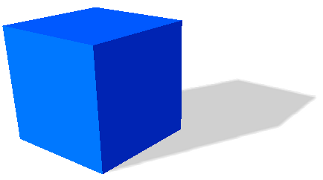
\includegraphics{boxshape.png}
        \label{fig:boxshape}
    \end{figure}

    The \texttt{BoxShape} class describes a box collision. The box is aligned with the shape local X, Y and Z axis.
    In order to create a box shape, you only need to specify the three half extents dimensions of the box in the three X, Y and Z directions. \\

    For instance, if you want to create a box shape with dimensions of 4 meters, 6 meters and 10 meters along the X, Y and Z axis respectively, you need to use the
    following code: \\

    \begin{lstlisting}
// Half extents of the box in the x, y and z directions
const rp3d::Vector3 halfExtents(2.0, 3.0, 5.0);

// Create the box shape
const rp3d::BoxShape boxShape(halfExtents);
  \end{lstlisting}

    \vspace{0.6cm}

    The \texttt{BoxShape} has a collision margin that is added to the box dimension you define. Therefore, the actual box shape will be a little bit larger that the one you define.
    It is recommended that you use the default margin. In case, you really need to change the collision margin of your box shape (if the dimension of your box is small compared
    to the default collision margin for instance), you can pass the length of the new collision margin (in meters) as a second parameter of the \texttt{BoxShape} constructor. \\

    For instance, if you want to use a collision margin of 1 centimeter for your box shape, you can do it like this: \\

   \begin{lstlisting}
// Create the box shape with a custom collision margin
const rp3d::BoxShape boxShape(halfExtents, 0.01);
  \end{lstlisting}

    \subsection{Sphere Shape}

    \begin{figure}[h]
        \centering
        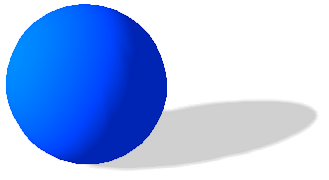
\includegraphics{sphereshape.png}
        \label{fig:sphereshape}
    \end{figure}

    The \texttt{SphereShape} class describes a sphere collision shape centered at the origin of the shape local space. You only need to specify the radius of the sphere to create it. \\

    For instance, if you want to create a sphere shape with a radius of 2 meters, you need to use the following code: \\

    \begin{lstlisting}
// Create the sphere shape with a radius of 2m
const rp3d::SphereShape sphereShape(2.0);
  \end{lstlisting}

    \vspace{0.6cm}

    The collision margin of the \texttt{SphereShape} is integrated into the sphere you define. Therefore, you do not need to worry about it and you cannot change it.

    \subsection{Cone Shape}

    \begin{figure}[h]
        \centering
        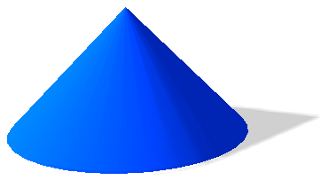
\includegraphics{coneshape.png}
        \label{fig:coneshape}
    \end{figure}

    The \texttt{ConeShape} class describes a cone collision shape centered at the origin of the shape local-space. The cone is aligned along the Y axis.
    In order to create a cone shape, you need to give the radius of its base and its height (along the Y axis). \\

    For instance, if you want to create a cone shape with a radius of 1 meter and the height of 3 meters, you need to use the following code: \\

    \begin{lstlisting}
// Create the cone shape
const rp3d::ConeShape coneShape(1.0, 3.0);
  \end{lstlisting}

    \vspace{0.6cm}

    The \texttt{ConeShape} has a collision margin that is added to the cone dimension that you define. Therefore, the actual cone shape will be a little bit larger that the size you define.
    It is recommended that you use the default margin. In case you really need to change the collision margin of your cone shape (if the dimension of your cone is small compared
    to the default collision margin for instance), you can pass the length of the new collision margin (in meters) as a third parameter of the \texttt{ConeShape} constructor. \\

    For instance, if you want to use a collision margin of 1 centimeter for your cone shape, you can do it like this: \\

   \begin{lstlisting}
// Create the cone shape with a custom collision margin
const rp3d::ConeShape coneShape(1.0, 3.0, 0.01);
  \end{lstlisting}

    \subsection{Cylinder Shape}

    \begin{figure}[h]
        \centering
        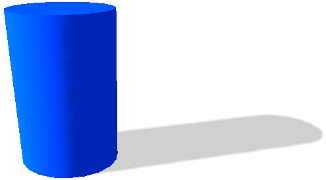
\includegraphics{cylindershape.png}
        \label{fig:cylindershape}
    \end{figure}

    The \texttt{CylinderShape} class describes a cylinder collision shape centered at the origin of the shape local-space. The cylinder is aligned along the Y axis.
    In order to create a cylinder shape, you need to specify the radius of its base and its height (along the Y axis). \\

    For instance, if you want to create a cylinder shape with a radius of 1 meter and the height of 3 meters, you need to use the following code: \\

    \begin{lstlisting}
// Create the cylinder shape
const rp3d::Cylinder cylinderShape(1.0, 3.0);
  \end{lstlisting}

    \vspace{0.6cm}

    The \texttt{CylinderShape} has a collision margin that is added to the cylinder dimension that you define. Therefore, the actual cylinder shape will be a little bit larger that the one you define.
    It is recommended that you use the default margin. In case you really need to change the collision margin of your cylinder shape (if the dimension of your cylinder is small compared
    to the default collision margin for instance), you can pass the length of the new collision margin (in meters) as a third parameter of the \texttt{CylinderShape} constructor. \\

    For instance, if you want to use a collision margin of 1 centimeter for your cylinder shape, you can do it like this: \\

   \begin{lstlisting}
// Create the cylinder shape with a custom collision margin
const rp3d::CylinderShape cylinderShape(1.0, 3.0, 0.01);
  \end{lstlisting}

    \subsection{Capsule Shape}

    \begin{figure}[h]
        \centering
        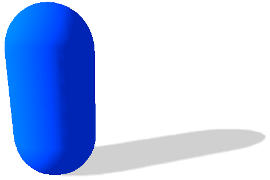
\includegraphics{capsuleshape.png}
        \label{fig:capsuleshape}
    \end{figure}

    The \texttt{CapsuleShape} class describes a capsule collision shape around the Y axis and centered at the origin of the shape local-space. It is the convex hull of two
    spheres. It can also be seen as an elongated sphere. In order to create it, you only need to specify the radius of the two spheres and the height of the
    capsule (distance between the centers of the two spheres).  \\

    For instance, if you want to create a capsule shape with a radius of 1 meter and the height of 2 meters, you need to use the following code: \\

    \begin{lstlisting}
// Create the capsule shape
const rp3d::CapsuleShape capsuleShape(1.0, 2.0);
  \end{lstlisting}

    \vspace{0.6cm}

    As for the \texttt{SphereShape}, the collision margin of the \texttt{CapsuleShape} is integrated into the capsule you define.
    Therefore, you do not need to worry about it and you cannot change it.

    \subsection{Convex Mesh Shape}

    \begin{figure}[h]
        \centering
        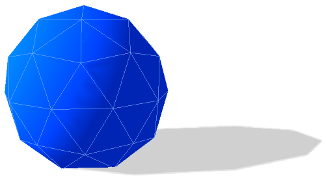
\includegraphics{convexshape.png}
        \label{fig:convexshape}
    \end{figure}

    The \texttt{ConvexMeshShape} class can be used to describe the shape of a convex mesh. In order to create a convex mesh shape, you need to supply the array with the coordinates of
    the vertices of the mesh. The array is supposed to start with the three X, Y and Z coordinates of the first vertex, then the X, Y and Z coordinates of the second vertex and so on.
    The first parameter of the \texttt{ConvexMeshShape} constructor is a pointer to the array of the vertices coordinates, the second parameter is the number of vertices in the array and
    the third parameter is the size (in bytes) of the data needed for a single vertex in the array (data used by all the three coordinates of a single vertex). \\

    The following example shows how to create a convex mesh shape: \\

    \begin{lstlisting}
// Construct a convex mesh shape
rp3d::ConvexMeshShape shape(verticesArray, nbVertices, 3 * sizeof(float));
  \end{lstlisting}

    \vspace{0.6cm}

    You need to make sure that the mesh you provide is indeed convex and also that the origin of its local-space is inside the mesh. \\

    The collision detection test with a convex mesh shape runs in $O(n)$ where $n$ is the number of vertices in the mesh. Collision detection can become expensive if there are
    too many vertices in the mesh. It is possible to speed up the collision detection by providing information about the edges of the convex mesh. If you provide edges information, the collision detection will run in almost constant time at the cost of a little extra memory to store the edges information. In order to provide the edges
    information, you need to call the \texttt{ConvexMeshShape::addEdge()} method for each edge of the mesh. The first parameter is the index of the first vertex of the edge and the
    second parameter is the index of the second vertex. Do not worry about calling this method multiple times for the same edge, the edge information will be added only
    once. \\

    For instance, the following code adds the edges information into a convex mesh shape: \\

    \begin{lstlisting}
// Add the edges information of the mesh into the shape
for (unsigned int i=0; i<mesh.getNbFaces(); i++) {

    // Get the three vertex IDs of the vertices of the face
    unsigned int v1 = getVertexIndexInFace(i, 0);
    unsigned int v2 = getVertexIndexInFace(i, 1);
    unsigned int v3 = getVertexIndexInFace(i, 2);

    // Add the three edges into the collision shape
    convexShape.addEdge(v1, v2);
    convexShape.addEdge(v1, v3);
    convexShape.addEdge(v2, v3);
}
  \end{lstlisting}

    \vspace{0.6cm}

    Do not forget to enable the fast collision detection by asking the collision shape to use the edges information you have just provided. To do this, you need to
    call the \texttt{ConvexMeshShape::setIsEdgesInformationUsed()} method as in the following example: \\

     \begin{lstlisting}
// Enable the fast collision detection
// using the edges information
collisionShape.setIsEdgesInformationUsed(true);
  \end{lstlisting}

  \subsection{Concave Mesh Shape}

  \begin{figure}[h]
      \centering
      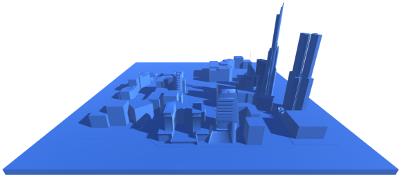
\includegraphics{concavemeshshape.png}
      \label{fig:concaveshape}
  \end{figure}

  The \texttt{ConcaveMeshShape} class can be used for a static concave triangular mesh. It can be used to describe an environment for
  instance. Note that it cannot be used with a dynamic body that is allowed to move. Moreover, make sure to use a \texttt{ConcaveMeshShape} only
  when you are not able to use a convex shape and also try to limit the number of triangles of that mesh because collision detection
  with \texttt{ConcaveMeshShape} is quite expensive compared to convex shapes. \\

  In order to create a concave mesh shape, you need to supply a pointer to a \texttt{TriangleMesh}. A \texttt{TriangleMesh} is a class
  that describes a mesh made of triangles. A \texttt{TriangleMesh} can contain several parts (submeshes). Each part is a set of
  triangles represented by a \texttt{TriangleVertexArray} object. First, you need to create a \texttt{TriangleVertexArray}. A \texttt{TriangleVertexArray} represents
  a continuous array of vertices and indexes for a triangular mesh. When you create a \texttt{TriangleVertexArray}, no data is copied
  into the array. It only stores a pointer to the data. The goal is to allow the user to share vertices data between the physics engine and the rendering
  part. Therefore, make sure that the data pointed by a \texttt{TriangleVertexArray} remains valid during the whole \texttt{TriangleVertexArray} life.
  \\

  The following example show how to create a \texttt{TriangleVertexArray}: \\

  \begin{lstlisting}
const int nbVertices = 8;
const int nbTriangles = 12;
float vertices[3 * nbVertices] = ...;
int indices[3 * nbTriangles] = ...;
rp3d::TriangleVertexArray* triangleArray =
new rp3d::TriangleVertexArray(nbVertices, vertices, 3 * sizeof(float), nbTriangles,
indices, sizeof(int),
rp3d::TriangleVertexArray::VERTEX_FLOAT_TYPE,
rp3d::TriangleVertexArray::INDEX_INTEGER_TYPE);
  \end{lstlisting}

  \vspace{0.6cm}

  Now that we have a \texttt{TriangleVertexArray}, we need to create a \texttt{TriangleMesh} and add the \texttt{TriangleVertexArray}
  into it as a subpart. Once this is done, we can create the actual \texttt{ConcaveMeshShape} and add it to the body we want to
  simulate as in the following example: \\

  \begin{lstlisting}
rp3d::TriangleMesh triangleMesh;

// Add the triangle vertex array to the triangle mesh
triangleMesh.addSubpart(triangleArray);

// Create the concave mesh shape
ConcaveMesh* concaveMesh = new rp3d::ConcaveMeshShape(&triangleMesh);
  \end{lstlisting}

  \vspace{0.6cm}

  Note that the \texttt{TriangleMesh} object also needs to exist during the whole life of the collision shape because its
  data is not copied into the collision shape.

  \subsection{Heightfield Shape}

  \begin{figure}[h]
      \centering
      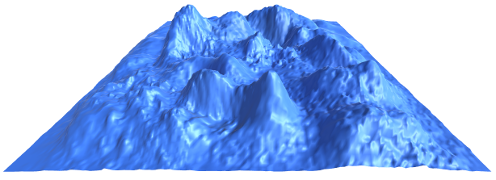
\includegraphics{heightfieldshape.png}
      \label{fig:heightfieldshape}
  \end{figure}

  The \texttt{HeightFieldShape} is a collision shape that can be used to represent a static terrain for instance. You can
  define a heightfield with a two dimensional grid that has a given height value at each point. \\

  In order to create a \texttt{HeightFieldShape}, you need to have an array with all the height values of your field.
  You can have height values of type int, float or double. You need to give the number of rows and columns of your two
  dimensional grid. Note that the height values in your array must be organized such that the value at row
  \texttt{indexRow} and column \texttt{indexColumn} is located at the following position in the array:

  \begin{lstlisting}
heighFieldValues[indexRow * nbColumns + indexColumn]
  \end{lstlisting}

  \vspace{0.6cm}

  Morevover, you need to provide the minimum and maximum height values of your height field. \\

  Here is an example that shows how to create a \texttt{HeightFieldShape}: \\

  \begin{lstlisting}
const int nbRows = 40;
const int nbColumns = 50;
float minHeight = 100;
float maxHeight = 500;

// Height values
float heightValues[nbRows * nbColumns] = ...;

// Create the heightfield collision shape
rp3d::HeightFieldShape = new rp3d::HeightFieldShape(nbColumns, nbRows, minHeight,
maxHeight, heightValues, rp3d::HeightFieldShape::HEIGHT_FLOAT_TYPE);
  \end{lstlisting}

  \vspace{0.6cm}

  Note that the array of height values is not copied into the \texttt{HeightFieldShape}. Therefore, you need to make sure
  it exists during the lifetime of the \texttt{HeightFieldShape} and you must not forget to release its memory when you
  destroy the collision shape or at the end of your application. \\

  When creating a \texttt{HeightFieldShape}, the origin of the shape will be at the center of its bounding volume.
  Therefore, if you create a \texttt{HeightFieldShape} with a minimum height of 100 and a maximum height of 500, the
  maximum coordinates of the shape on the Y axis will be 200 and the minimum coordinates will be -200.

    \subsection{Adding a Collision Shape to a body - The Proxy Shape concept}

    \begin{sloppypar}
    Now that you know how to create a collision shape, we will see how to add it to a given body. \\

    First note that when you add a collision shape to a body, the shape will not be copied internally. You only give a
    pointer to the shape in parameter. The shape must exist during the whole lifetime of the body. This way, you can
    create a collision shape and reuse it for multiple bodies. You are also responsible to destroy the shape at the
    end when the bodies are not used anymore. \\

   In order to add a collision shape to a body, you need to use the \texttt{CollisionBody::addCollisionShape()} method for a Collision Body and the
   \texttt{RigidBody::addCollisionShape()} method for a Rigid Body. You will have to provide the collision shape transform in parameter. This is the
   transformation mapping the local-space of the collision shape to the local-space of the body. For a Rigid Body, you will also have to provide the
   mass of the shape you want to add. As explained before, this is used to automatically compute the center of mass, total mass and inertia tensor of the body. \\

   The \texttt{addCollisionShape()} method returns a pointer to a Proxy Shape. A Proxy Shape is what links a given collision shape to the body it has been added.
   You can use the returned Proxy Shape to get or set parameters of the given collision shape in that particular body. This concept is also called \emph{fixture} in some
   other physics engines. In ReactPhysics3D, a Proxy Shape is represented by the \texttt{ProxyShape} class. \\

    The following example shows how to add a sphere collision shape with a given mass to a rigid body and also how to remove it from the body using the Proxy Shape pointer. \\
    \end{sloppypar}

    \begin{lstlisting}
// Create the sphere collision shape
rp3d::decimal radius = rp3d::decimal(3.0)
const rp3d::BoxShape shape(radius);

// Transform of the collision shape
// Place the shape at the origin of the body local-space
rp3d::Transform transform = rp3::Transform::identity();

// Mass of the collision shape (in kilograms)
rp3d::decimal mass = rp3d::decimal(4.0);

// Add the collision shape to the rigid body
rp3d::ProxyShape* proxyShape;
proxyShape = body->addCollisionShape(&shape, transform, mass);

// If you want to remove the collision shape from the body
// at some point, you need to use the proxy shape
body->removeCollisionShape(proxyShape);
  \end{lstlisting}

    \vspace{0.6cm}

    As you can see, you can use the \texttt{removeCollisionShape()} method to remove a collision shape from a body by using the Proxy Shape. Note that
    after removing a collision shape, the corresponding Proxy Shape pointer will not be valid anymore. It is not necessary to manually remove all the collision shapes from
    a body at the end of your application. They will automatically be removed when you destroy the body.

    \subsection{Collision filtering}
    \label{sec:collisionfiltering}

    By default all the collision shapes of all your bodies are able to collide with each other in the world. However, sometimes we want a body to collide only with a given
    group of bodies and not with other bodies. This is called collision filtering. The idea is to group the collision shapes of bodies into categories. Then we can specify
    for each collision shape against which categories it will be able to collide. \\

    ReactPhysics3D uses bits mask to represent categories. The first thing to do is to assign a category to the collision shapes of your body. To do this, you need to
    call the \texttt{ProxyShape::setCollisionCategoryBits()} method on the corresponding Proxy Shape as in the following example. Here we consider that we have four bodies
    where each one has a single collision shape. \\

    \begin{lstlisting}
// Enumeration for categories
enum Category {
   CATEGORY1 = 0x0001,
   CATEGORY2 = 0x0002,
   CATEGORY3 = 0x0004
};


// Set the collision category for each proxy shape of
// each of the four bodies
proxyShapeBody1->setCollisionCategoryBits(CATEGORY1);
proxyShapeBody2->setCollisionCategoryBits(CATEGORY2);
proxyShapeBody3->setCollisionCategoryBits(CATEGORY3);
proxyShapeBody4->setCollisionCategoryBits(CATEGORY3);
  \end{lstlisting}

    \vspace{0.6cm}

    As you can see, the collision shape of body 1 will be part of the category 1, the collision shape of body 2 will be part of the category 2 and the collision shapes of bodies 3 and 4 will be
    part of the category 3. \\

    \begin{sloppypar}
    Now, for each collision shape, we need to specify with which categories the shape is allowed to collide with. To do this, you need to use the \texttt{ProxyShape::setCollideWithMaskBits()}
    method of the Proxy Shape. Note that you can specify one or more categories using the bitwise OR operator. The following example shows how to specify with which categories the
    shapes can collide. \\
    \end{sloppypar}

    \begin{lstlisting}
// For each shape, we specify with which categories it
// is allowed to collide
proxyShapeBody1->setCollideWithMaskBits(CATEGORY3);
proxyShapeBody2->setCollideWithMaskBits(CATEGORY1 | CATEGORY3);
proxyShapeBody3->setCollideWithMaskBits(CATEGORY2);
proxyShapeBody4->setCollideWithMaskBits(CATEGORY2);
  \end{lstlisting}

    \vspace{0.6cm}

    As you can see, we specify that the body 1 will be allowed to collide with bodies from the categorie 3. We also indicate that the body 2 will be allowed to collide with bodies from the
    category 1 and 3 (using the bitwise OR operator). Finally, we specify that bodies 3 and 4 will be allowed to collide against bodies of the category 2. \\

    A collision shape is able to collide with another only if you have specify that the category mask of the first shape is part of the \emph{collide with} mask of the second shape. It
    is also important to understand that this condition must be satisfied in both directions. For instance in the previous example, the body 1 (of category 1) says that it wants to collide
    against bodies of the category 3 (for instance against body 3). However, body 1 and body 3 will not be able to collide because the body 3 does not say that it wants to collide
    with bodies from category 1. Therefore, in the previous example, the body 2 is allowed to collide against bodies 3 and 4 but no other collision is allowed. \\

    In the same way, you can perform this filtering for ray casting (described in section \ref{sec:raycasting}). For instance, you can perform a ray cast test
    against a given subset of categories of collision shapes only.

    \section{Joints}

    Joints are used to constraint the motion of the rigid bodies between each other. A single joint represents a constraint between two rigid bodies.
    When the motion of the first body of the joint is known, the relative motion of the second body has at most six degrees of freedom (three for the
    translation and three for the rotation). The different joints can reduce the number of degrees of freedom between two rigid bodies. \\

    Some joints have limits to control the range of motion and some joints have motors to automatically move the bodies of the joint at a given speed. \\

    \subsection{Ball and Socket Joint}

    The \texttt{BallAndSocketJoint} class describes a ball and socket joint between two bodies. In a ball and socket joint, the two bodies cannot translate with respect to each other.
    However, they can rotate freely around a common anchor point. This joint has three degrees of freedom and can be used to simulate a chain of bodies for instance. \\

    In order to create a ball and socket joint, you first need to create an instance of the \texttt{BallAndSocketJointInfo} class with the necessary information. You need to provide the pointers to the
    two rigid bodies and also the coordinates of the anchor point (in world-space). At the joint creation, the world-space anchor point will be converted into the local-space of the two rigid
    bodies and then, the joint will make sure that the two local-space anchor points match in world-space. Therefore, the two bodies need to be in a correct position at the joint creation. \\

    Here is the code to create the \texttt{BallAndSocketJointInfo} object: \\

    \begin{lstlisting}
// Anchor point in world-space
const rp3d::Vector3 anchorPoint(2.0, 4.0, 0.0);

// Create the joint info object
rp3d::BallAndSocketJointInfo jointInfo(body1, body2, anchorPoint);
  \end{lstlisting}

    \vspace{0.6cm}

    Now, it is time to create the actual joint in the dynamics world using the \texttt{DynamicsWorld::createJoint()} method.
    Note that this method will also return a pointer to the \texttt{BallAndSocketJoint} object that has been created internally. You will then
    be able to use that pointer to change properties of the joint and also to destroy it at the end. \\

    Here is how to create the joint in the world: \\

    \begin{lstlisting}
// Create the joint in the dynamics world
rp3d::BallAndSocketJoint* joint;
joint = dynamic_cast<rp3d::BallAndSocketJoint*>(world.createJoint(jointInfo));
  \end{lstlisting}

    \vspace{0.6cm}

    \subsection{Hinge Joint}

    The \texttt{HingeJoint} class describes a hinge joint (or revolute joint) between two rigid bodies. The hinge joint only allows rotation around an anchor point and
    around a single axis (the hinge axis). This joint can be used to simulate doors or pendulums for instance. \\

    In order to create a hinge joint, you first need to create a \texttt{HingeJointInfo} object with the necessary information. You need to provide the pointers to the
    two rigid bodies, the coordinates of the anchor point (in world-space) and also the hinge rotation axis (in world-space). The two bodies need to be in a correct position
    when the joint is created. \\

    Here is the code to create the \texttt{HingeJointInfo} object: \\

    \begin{lstlisting}
// Anchor point in world-space
const rp3d::Vector3 anchorPoint(2.0, 4.0, 0.0);

// Hinge rotation axis in world-space
const rp3d::Vector3 axis(0.0, 0.0, 1.0);

// Create the joint info object
rp3d::HingeJointInfo jointInfo(body1, body2, anchorPoint, axis);
  \end{lstlisting}

    \vspace{0.6cm}

    Now, it is time to create the actual joint in the dynamics world using the \texttt{DynamicsWorld::createJoint()} method.
    Note that this method will also return a pointer to the \texttt{HingeJoint} object that has been created internally. You will then
    be able to use that pointer to change properties of the joint and also to destroy it at the end. \\

    Here is how to create the joint in the world: \\

    \begin{lstlisting}
// Create the hinge joint in the dynamics world
rp3d::HingeJoint* joint;
joint = dynamic_cast<rp3d::HingeJoint*>(world.createJoint(jointInfo));
  \end{lstlisting}

     \subsubsection{Limits}

     With the hinge joint, you can constrain the motion range using limits. The limits of the hinge joint are the minimum and maximum angle of rotation allowed with respect to the initial
     angle between the bodies when the joint is created. The limits are disabled by default. If you want to use the limits, you first need to enable them by setting the
     \texttt{isLimitEnabled} variable of the \texttt{HingeJointInfo} object to \emph{true} before you create the joint. You also have to specify the minimum and maximum limit
     angles (in radians) using the \texttt{minAngleLimit} and \texttt{maxAngleLimit} variables of the joint info object. Note that the minimum limit angle must be in the
     range $[ -2 \pi; 0 ]$ and the maximum limit angle must be in the range $[ 0; 2 \pi ]$. \\

     For instance, here is the way to use the limits for a hinge joint when the joint is created: \\

     \begin{lstlisting}
// Create the joint info object
rp3d::HingeJointInfo jointInfo(body1, body2, anchorPoint, axis);

// Enable the limits of the joint
jointInfo.isLimitEnabled = true;

// Minimum limit angle
jointInfo.minAngleLimit = -PI / 2.0;

// Maximum limit angle
jointInfo.maxAngleLimit = PI / 2.0;

// Create the hinge joint in the dynamics world
rp3d::HingeJoint* joint;
joint = dynamic_cast<rp3d::HingeJoint*>(world.createJoint(jointInfo));
  \end{lstlisting}

     \vspace{0.6cm}

     \begin{sloppypar}
        It is also possible to use the \texttt{HingeJoint::enableLimit()}, \texttt{HingeJoint::setMinAngleLimit()} and \texttt{HingeJoint::setMaxAngleLimit()} methods to specify
        the limits of the joint after its creation. See the API documentation for more information.
     \end{sloppypar}

     \subsubsection{Motor}

     A motor is also available for the hinge joint. It can be used to rotate the bodies around the hinge axis at a given angular speed and such that the torque applied to
     rotate the bodies does not exceed a maximum allowed torque. The motor is disabled by default. If you want to use it, you first have to activate it using the
     \texttt{isMotorEnabled} boolean variable of the \texttt{HingeJointInfo} object before you create the joint. Then, you need to specify the angular motor speed (in radians/seconds)
     using the \texttt{motorSpeed} variable and also the maximum allowed torque (in Newton $\cdot$ meters) with the \texttt{maxMotorTorque} variable. \\

     For instance, here is how to enable the motor of the hinge joint when the joint is created: \\

     \begin{lstlisting}
// Create the joint info object
rp3d::HingeJointInfo jointInfo(body1, body2, anchorPoint, axis);

// Enable the motor of the joint
jointInfo.isMotorEnabled = true;

// Motor angular speed
jointInfo.motorSpeed = PI / 4.0;

// Maximum allowed torque
jointInfo.maxMotorTorque = 10.0;

// Create the hinge joint in the dynamics world
rp3d::HingeJoint* joint;
joint = dynamic_cast<rp3d::HingeJoint*>(world.createJoint(jointInfo));
  \end{lstlisting}

     \vspace{0.6cm}

     \begin{sloppypar}
        It is also possible to use the \texttt{HingeJoint::enableMotor()}, \texttt{HingeJoint::setMotorSpeed()} and \texttt{HingeJoint::setMaxMotorTorque()} methods to
        enable the motor of the joint after its creation. See the API documentation for more information.
     \end{sloppypar}

    \subsection{Slider Joint}

    The \texttt{SliderJoint} class describes a slider joint (or prismatic joint) that only allows relative translation along a single direction. It has a single degree of freedom and allows no
    relative rotation. In order to create a slider joint, you first need to specify the anchor point (in world-space) and the slider axis direction (in world-space). The constructor of the
    \texttt{SliderJointInfo} object needs two pointers to the bodies of the joint, the anchor point and the axis direction. Note that the two bodies have to be in a correct initial position when
    the joint is created. \\

    You can see in the following code how to specify the information to create a slider joint: \\

    \begin{lstlisting}
// Anchor point in world-space
const rp3d::Vector3 anchorPoint = rp3d::decimal(0.5) * (body2Position + body1Position);

// Slider axis in world-space
const rp3d::Vector3 axis = (body2Position - body1Position);

// Create the joint info object
rp3d::SliderJointInfo jointInfo(body1, body2, anchorPoint, axis);
  \end{lstlisting}

    \vspace{0.6cm}

    Now, it is possible to create the actual joint in the dynamics world using the \texttt{DynamicsWorld::createJoint()} method.
    Note that this method will also return a pointer to the \texttt{SliderJoint} object that has been created internally. You will then
    be able to use that pointer to change properties of the joint and also to destroy it at the end. \\

    Here is how to create the joint in the world: \\

    \begin{lstlisting}
// Create the slider joint in the dynamics world
rp3d::SliderJoint* joint;
joint = dynamic_cast<rp3d::SliderJoint*>(world.createJoint(jointInfo));
  \end{lstlisting}

    \subsubsection{Limits}

    It is also possible to control the range of the slider joint motion using limits. The limits are disabled by default. In order to use the limits when the joint is created, you first
    need to activate them using the \texttt{isLimitEnabled} variable of the \texttt{SliderJointInfo} class. Then, you need to specify the minimum and maximum translation limits
    (in meters) using the \texttt{minTranslationLimit} and \texttt{maxTranslation\-Limit} variables. Note that the initial position of the two bodies when the joint is created
    corresponds to a translation of zero. Therefore, the minimum limit must be smaller or equal to zero and the maximum limit must be larger or equal to zero. \\

    You can see in the following example how to set the limits when the slider joint is created: \\

    \begin{lstlisting}
// Create the joint info object
rp3d::SliderJointInfo jointInfo(body1, body2, anchorPoint, axis);

// Enable the limits of the joint
jointInfo.isLimitEnabled = true;

// Minimum translation limit
jointInfo.minTranslationLimit = -1.7;

// Maximum translation limit
jointInfo.maxTranslationLimit = 1.7;

// Create the hinge joint in the dynamics world
rp3d::SliderJoint* joint;
joint = dynamic_cast<rp3d::SliderJoint*>(world.createJoint(jointInfo));
  \end{lstlisting}

    \vspace{0.6cm}

   \begin{sloppypar}
     You can also use the \texttt{SliderJoint::enableLimit()}, \texttt{SliderJoint::\-setMinTranslationLimit()} and \texttt{SliderJoint::setMaxTranslationLimit()} methods to
     enable the limits of the joint after its creation. See the API documentation for more information.
    \end{sloppypar}

    \subsubsection{Motor}

     The slider joint also has a motor. You can use it to translate the bodies along the slider axis at a given linear speed and such that the force applied to
     move the bodies does not exceed a maximum allowed force. The motor is disabled by default. If you want to use it when the joint is created, you first have to activate it using the
     \texttt{isMotorEnabled} boolean variable of the \texttt{SliderJointInfo} object before you create the joint. Then, you need to specify the linear motor speed (in meters/seconds)
     using the \texttt{motorSpeed} variable and also the maximum allowed force (in Newtons) with the \texttt{maxMotorForce} variable. \\

     For instance, here is how to enable the motor of the slider joint when the joint is created: \\

     \begin{lstlisting}
// Create the joint info object
rp3d::SliderJointInfo jointInfo(body1, body2, anchorPoint, axis);

// Enable the motor of the joint
jointInfo.isMotorEnabled = true;

// Motor linear speed
jointInfo.motorSpeed = 2.0;

// Maximum allowed force
jointInfo.maxMotorForce = 10.0;

// Create the slider joint in the dynamics world
rp3d::SliderJoint* joint;
joint = dynamic_cast<rp3d::SliderJoint*>(world.createJoint(jointInfo));
  \end{lstlisting}

     \vspace{0.6cm}

     \begin{sloppypar}
        It is also possible to use the \texttt{SliderJoint::enableMotor()}, \texttt{SliderJoint::setMotorSpeed()} and \texttt{SliderJoint::setMaxMotorForce()} methods to enable the
        motor of the joint after its creation. See the API documentation for more information.
     \end{sloppypar}

    \subsection{Fixed Joint}

    The \texttt{FixedJoint} class describes a fixed joint between two bodies. In a fixed joint, there is no degree of freedom, the bodies are not allowed to translate
    or rotate with respect to each other. In order to create a fixed joint, you simply need to specify an anchor point (in world-space) to create the \texttt{FixedJointInfo}
    object. \\

    For instance, here is how to create the joint info object for a fixed joint: \\

    \begin{lstlisting}
// Anchor point in world-space
rp3d::Vector3 anchorPoint(2.0, 3.0, 4.0);

// Create the joint info object
rp3d::FixedJointInfo jointInfo1(body1, body2, anchorPoint);
  \end{lstlisting}

    \vspace{0.6cm}

    Now, it is possible to create the actual joint in the dynamics world using the \texttt{DynamicsWorld::createJoint()} method.
    Note that this method will also return a pointer to the \texttt{FixedJoint} object that has been created internally. You will then
    be able to use that pointer to change properties of the joint and also to destroy it at the end. \\

    Here is how to create the joint in the world: \\

    \begin{lstlisting}
// Create the fixed joint in the dynamics world
rp3d::FixedJoint* joint;
joint = dynamic_cast<rp3d::FixedJoint*>(world.createJoint(jointInfo));
  \end{lstlisting}

    \subsection{Collision between the bodies of a Joint}

    By default the two bodies involved in a joint are able to collide with each other. However, it is possible to disable the collision between the two bodies that are part
    of the joint. To do it, you simply need to set the variable \texttt{isCollisionEnabled} of the joint info object to \emph{false} when you create the joint. \\

    For instance, when you create a \texttt{HingeJointInfo} object in order to construct a hinge joint, you can disable the collision between the two bodies of the joint as in the
    following example: \\

    \begin{lstlisting}
// Create the joint info object
rp3d::HingeJointInfo jointInfo(body1, body2, anchorPoint, axis);

// Disable the collision between the bodies
jointInfo.isCollisionEnabled = false;

// Create the joint in the dynamics world
rp3d::HingeJoint* joint;
joint = dynamic_cast<rp3d::HingeJoint*>(world.createJoint(jointInfo));
  \end{lstlisting}

    \subsection{Destroying a Joint}

    \begin{sloppypar}
    In order to destroy a joint, you simply need to call the \texttt{DynamicsWorld::destroyJoint()} method using the pointer to
    a previously created joint object as argument as shown in the following code: \\
   \end{sloppypar}

    \begin{lstlisting}
// rp3d::BallAndSocketJoint* joint is a previously created joint

// Destroy the joint
world.destroyJoint(joint);
  \end{lstlisting}

    \vspace{0.6cm}

    It is important that you destroy all the joints that you have created at the end of the simulation. Also note that destroying a
    rigid body involved in a joint will automatically destroy that joint.

    \section{Ray casting}
    \label{sec:raycasting}

    You can use ReactPhysics3D to test intersection between a ray and the bodies of the world you have created. Ray casting can be performed against multiple bodies, a single body or
    any proxy shape of a given body. \\

    The first thing you need to do is to create a ray using the \texttt{Ray} class of ReactPhysics3D. As you can see in the following example, this is very easy. You
    simply need to specify the point where the ray starts and the point where the ray ends (in world-space coordinates). \\

    \begin{lstlisting}
// Start and end points of the ray
rp3d::Vector3 startPoint(0.0, 5.0, 1.0);
rp3d::Vector3 endPoint(0.0, 5.0, 30);

// Create the ray
rp3d::Ray ray(startPoint, endPoint);
  \end{lstlisting}

    \vspace{0.6cm}

    Any ray casting test that will be described in the following sections returns a \texttt{RaycastInfo} object in case of intersection with the ray.
    This structure contains the following attributes: \\

    \begin{description}
         \item[worldPoint] Hit point in world-space coordinates
         \item[worldNormal] Surface normal of the proxy shape at the hit point in world-space coordinates
         \item[hitFraction] Fraction distance of the hit point between \emph{startPoint}  and \emph{endPoint} of the ray. The hit point \emph{p} is such that
           $p = startPoint + hitFraction \cdot (endPoint - startPoint)$
         \item[body] Pointer to the Collision Body or Rigid Body that has been hit by the ray
         \item[proxyShape] Pointer to the Proxy Shape that has been hit by the ray
    \end{description}

    Note that you can also use collision filtering with ray casting in order to only test ray intersection with specific proxy shapes.
    Collision filtering is described in section \ref{sec:collisionfiltering}.

    \subsection{Ray casting against multiple bodies}

    This ray casting query will return all the proxy shapes of all bodies in the world that are intersected by a given ray.

    \subsubsection{The RaycastCallback class}

    First, you have to implement your own class that inherits from the \texttt{RaycastCallback} class. Then, you need to override the
    \texttt{RaycastCallback::notifyRaycastHit()} method in your own class. An instance of your class have to be provided as a parameter
    of the raycast method and the \texttt{notifyRaycastHit()} method will be called for each proxy shape that is hit by the ray. You will receive, as a parameter
    of this method, a \texttt{RaycastInfo} object that will contain the information about the raycast hit (hit point, hit surface normal, hit body, hit proxy shape, \dots). \\

    In your \texttt{notifyRaycastHit()} method, you need to return a fraction value that will specify the continuation of the ray cast after a hit.
    The return value is the next maxFraction value to use. If you return a fraction of 0.0, it means that the raycast should terminate. If you return a
    fraction of 1.0, it indicates that the ray is not clipped and the ray cast should continue as if no hit occurred. If you return the fraction in the
    parameter (hitFraction value in the \texttt{RaycastInfo} object), the current ray will be clipped to this fraction in the next queries. If you return -1.0, it will
    ignore this ProxyShape and continue the ray cast. Note that no assumption can be done about the order of the calls of the \texttt{notifyRaycastHit()} method. \\

    Here is an example about creating your own raycast callback class that inherits from the \texttt{RaycastCallback} class and how to override the
    \texttt{notifyRaycastHit()} method: \\

    \begin{lstlisting}
// Class WorldRaycastCallback
class MyCallbackClass : public rp3d::RaycastCallback {

public:

   virtual decimal notifyRaycastHit(const RaycastInfo& info) {

      // Display the world hit point coordinates
      std::cout << "Hit point : " <<
                    info.worldPoint.x <<
                    info.worldPoint.y <<
                    info.worldPoint.z <<
                    std::endl;

      // Return a fraction of 1.0 to gather all hits
      return decimal(1.0);
    }
};
  \end{lstlisting}

    \subsubsection{Raycast query in the world}

    Now that you have your own raycast callback class, you can use the \texttt{raycast()} method to perform a ray casting test
    on a Collision World or a Dynamics World. \\

    The first parameter of this method is a reference to the \texttt{Ray} object representing the ray you need to test intersection with. The second parameter is a pointer to
    the object of your raycast callback object. You can specify an optional third parameter which is the bit mask for collision filtering.
    It can be used to raycast only against selected categories of proxy shapes as described in section \ref{sec:collisionfiltering}. \\

    \begin{lstlisting}
// Create the ray
rp3d::Vector3 startPoint(1 , 2, 10);
rp3d::Vector3 endPoint(1, 2, -20);
Ray ray(startPoint, endPoint);

// Create an instance of your callback class
MyCallbackClass callbackObject;

// Raycast test
world->raycast(ray, &callbackObject);
    \end{lstlisting}

    \vspace{0.6cm}

    \subsection{Ray casting against a single body}

    \begin{sloppypar}

    You can also perform ray casting against a single specific Collision Body or Rigid Body of the world. To do this, you need to use the
    \texttt{CollisionBody::raycast()} method. This method takes two parameters. The first one is a reference to the \texttt{Ray} object and the second one
    is a reference to the \texttt{RaycastInfo} object that will contain hit information if the ray hits the body. This method returns true if the ray hits the
    body. The \texttt{RaycastInfo} object will only be valid if the returned value is \emph{true} (a hit occured). \\

    \end{sloppypar}

    The following example shows how test ray intersection with a body: \\

    \begin{lstlisting}
// Create the ray
rp3d::Vector3 startPoint(1 , 2, 10);
rp3d::Vector3 endPoint(1, 2, -20);
Ray ray(startPoint, endPoint);

// Create the raycast info object for the
// raycast result
RaycastInfo raycastInfo;

// Raycast test
bool isHit = body->raycast(ray, raycastInfo);
    \end{lstlisting}

    \vspace{0.6cm}

    \subsection{Ray casting against the proxy shape of a body}

    You can also perform ray casting against a single specific Proxy Shape of a Collision Body or Rigid Body of the world. To do this, you need to use the
    \texttt{ProxyShape::raycast()} method of the given Proxy Shape. This method takes two parameters. The first one is a reference to the \texttt{Ray}
    object and the second one is a reference to the \texttt{RaycastInfo} object that will contain hit information if the ray hits the body. This method returns
    true if the ray hits the body. The \texttt{RaycastInfo} object will only be valid if the returned value is \emph{true} (a hit occured). \\

    The following example shows how to test ray intersection with a given Proxy Shape: \\

    \begin{lstlisting}
// Create the ray
rp3d::Vector3 startPoint(1 , 2, 10);
rp3d::Vector3 endPoint(1, 2, -20);
Ray ray(startPoint, endPoint);

// Create the raycast info object for the
// raycast result
RaycastInfo raycastInfo;

// Test raycasting against a proxy shape
bool isHit = proxyShape->raycast(ray, raycastInfo);
    \end{lstlisting}

    \vspace{0.6cm}

    \section{Testbed application}
    \label{sec:testbed}

    \begin{figure}[h]
        \centering
        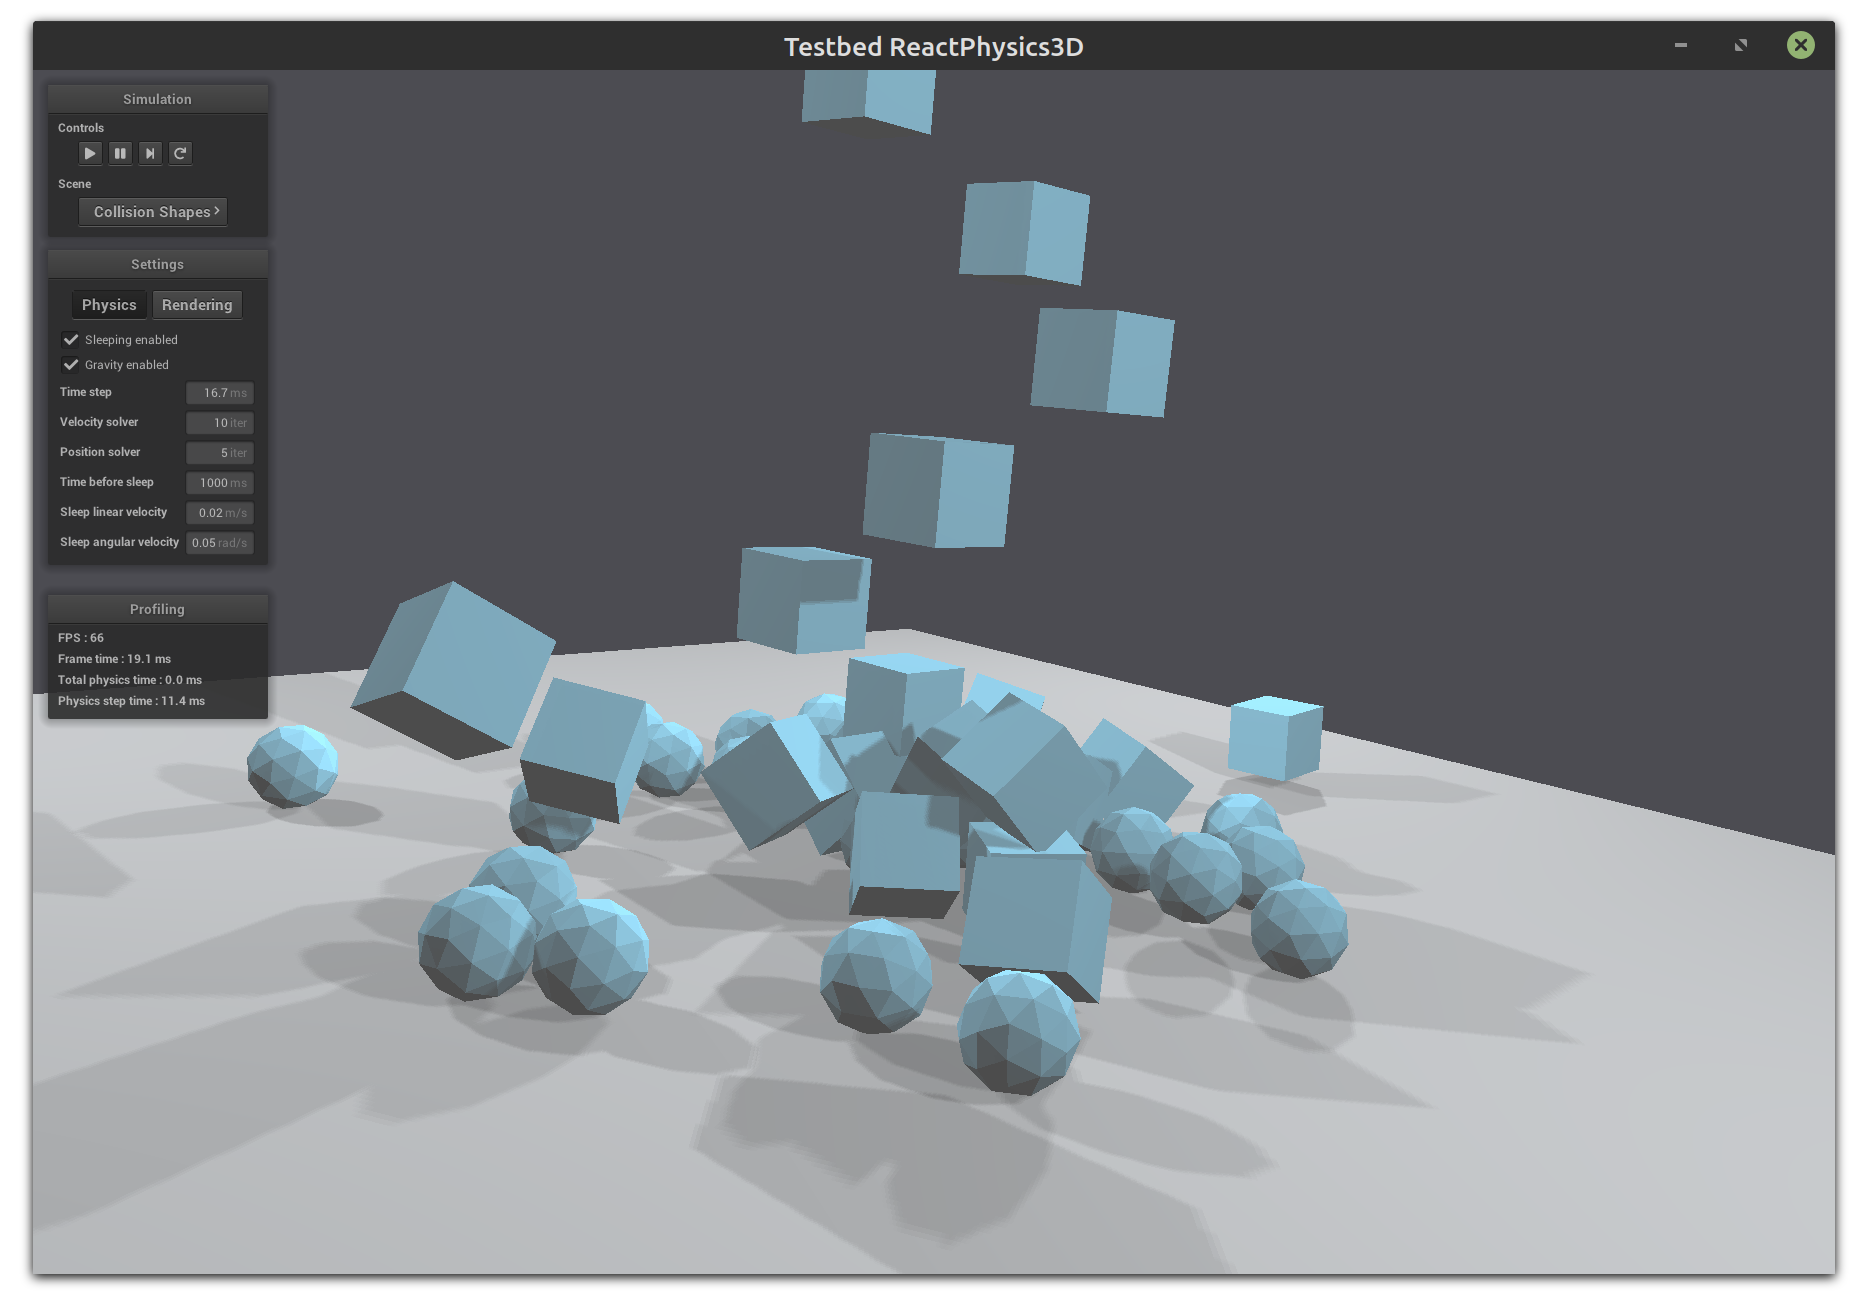
\includegraphics{testbed.png}
        \label{fig:testbed}
    \end{figure}

    The testbed application is a graphical interface where you can select and see some demo scenes using the
    ReactPhysics3D library. \\

    Follow the instructions described in section \ref{sec:building} to
    compile the testbed application. Note that OpenGL is required to compile it. \\

    The testbed application can be found in the \texttt{testbed/} folder of
    the ReactPhysics3D library. Do not hesitate to take a look at the code of the demo scenes to better understand how
    to use the library in your application. \\

    The following subsections describe the demo scenes that can be found in the testbed application.

    \subsection{Cubes Scene}

    In this scene, you will see how to create a floor and some cubes using the Box Shape for collision detection. Because of gravity,
    the cubes will fall down on the floor. After falling down, the cubes will come to rest and start sleeping (become inactive). In this scene,
    the cubes will become red as they get inactive (sleeping).

    \subsection{Joints}

    In this scene, you will learn how to create different joints (Ball and Socket, Hinge, Slider, Fixed) into the dynamics world. You can also see how
    to set the motor or limits of the joints.

    \subsection{Collision Shapes Scene}

    In this scene, you will see how to create a floor (using the Box Shape) and some other bodies using the different collision shapes available
    in the ReactPhysics3D library like Cylinders, Capsules, Spheres, Convex Meshes and Cones. Those bodies will fall down to the floor.

    \subsection{Heightfield Scene}

    In this scene, you will see how to use the Height field collision shape of the library. Several cubes will fall
    down to the height field.

    \subsection{Raycast Scene}

    In this scene, you will see how to use the ray casting methods of the library. Several rays are thrown against the different collision shapes.
    It is possible to switch from a collision shape to another using the spacebar key.

    \subsection{Concave Mesh Scene}

    In this scene, you will see how to use the static concave mesh collision shape of the library.

    \section{Retrieving contacts}

    There are several ways to get the contacts information (contact point, normal, penetration depth, \dots) from the \texttt{DynamicsWorld}. \\

    \subsection{Contacts of a given rigid body}

    If you are interested to retrieve all the contacts of a single rigid body, you can use the \texttt{RigidBody::getContactManifoldsList()} method. This method will
    return a linked list with all the current contact manifolds of the body. A contact manifold can contains several contact points. \\

    Here is an example showing how to get the contact points of a given rigid body: \\

    \begin{lstlisting}
const ContactManifoldListElement* listElem;

// Get the head of the linked list of contact manifolds of the body
listElem = rigidbody->getContactManifoldsList();

// For each contact manifold of the body
for (; listElem != NULL; listElem = listElem->next) {
    ContactManifold* manifold = listElem->contactManifold;

    // For each contact point of the manifold
    for (int i=0; i<manifold->getNbContactPoints(); i++) {

        // Get the contact point
        ContactPoint* point = manifold->getContactPoint(i);

        // Get the world-space contact point on body 1
        Vector3 pos = point->getWorldPointOnBody1();

        // Get the world-space contact normal
        Vector3 normal = point->getNormal();
    }
}
    \end{lstlisting}

     \vspace{0.6cm}

    Note that this technique to retrieve the contacts, if you use it between the \texttt{DynamicsWorld::update()} calls, will only give you the contacts are the end of
    each frame. You will probably miss several contacts that have occured in the physics internal sub-steps. In section \ref{sec:receiving_feedback}, you will
    see how to get all the contact occuring in the physis sub-steps of the engine. Also note that a contact manifold contains some persistent contact points that
    have may have been there for several frames.

    \subsection{All the contacts of the world}

    If you want to retrieve all the contacts of any rigid body in the world, you can use the \texttt{DynamicsWorld::getContactsList()} method. This method will
    a \texttt{std::vector} with the list of all the current contact manifolds of the world. A contact manifold may contain several contact points. \\

    The following example shows how to get all the contacts of the world using this method: \\

    \begin{lstlisting}
std::vector<ContactManifold*> manifolds;

// Get all the contacts of the world
manifolds = dynamicsWorld->getContactsList();
std::vector<ContactManifold*>::iterator it;

// For each contact manifold of the body
for (it = manifolds.begin(); it != manifolds.end(); ++it) {
    ContactManifold* manifold = *it;

    // For each contact point of the manifold
    for (int i=0; i<manifold->getNbContactPoints(); i++) {

        // Get the contact point
        ContactPoint* point = manifold->getContactPoint(i);

        // Get the world-space contact point on body 1
        Vector3 pos = point->getWorldPointOnBody1();

        // Get the world-space contact normal
        Vector3 normal = point->getNormal();
    }
}
    \end{lstlisting}

     \vspace{0.6cm}

    Note that this technique to retrieve the contacts, if you use it between the \texttt{DynamicsWorld::update()} calls, will only give you the contacts are the end of
    each frame. You will probably miss several contacts that have occured in the physics internal sub-steps. In section \ref{sec:receiving_feedback}, you will
    see how to get all the contact occuring in the physis sub-steps of the engine. Also note that a contact manifold contains some persistent contact points that
    have may have been there for several frames.

    \section{Receiving Feedback}
    \label{sec:receiving_feedback}
    Sometimes, you want to receive notifications from the physics engine when a given event happens. The \texttt{EventListener} class can be used for that purpose. In order to use
    it, you need to create a new class that inherits from the \texttt{EventListener} class and overrides some methods that will be called by the ReactPhysics3D library when some events
    occur. You also need to register your class in the physics world using the \texttt{DynamicsWorld::setEventListener()} as in the following code: \\

    \begin{lstlisting}
// Here, YourEventListener is a class that inherits
// from the EventListener class of reactphysics3d
YourEventListener listener;

// Register your event listener class
world.setEventListener(&listener);
  \end{lstlisting}

    \subsection{Contacts}

   If you want to be notified when two bodies that were separated before become in contact, you need to override the \texttt{EventListener::beginContact()} method in your event
   listener class. Then, this method will be called when the two separated bodies becomes in contact. \\

   If you receive a notification when a new contact between two bodies is found, you need to override the \texttt{EventListener::newContact()} method in your event listener class. Then, this
   method will be called when a new contact is found.

    \section{Profiler}

    If you build the library with the \texttt{PROFILING\_ENABLED} variable enabled (see section \ref{sec:cmakevariables}), a real-time profiler will collect information while the application
    is running. Then, at the end of your application, when the destructor of the \texttt{DynamicsWorld} class is called, information about the running time of the library will be displayed in the
    standard output. This can be useful to know where time is spent in the different parts of the ReactPhysics3D library in case your application is too slow.

   \section{API Documentation}

   Some documentation about the API of the code has been generated
   using Doxygen. You will be able to find this documentation in the library archive in the folder \texttt{/documentation/API/html/}. You just
   need to open the \texttt{index.html} file with your favorite web browser.

    \section{Bugs}

    If you find some bugs, do not hesitate to report them on our issue tracker here: \\

    \url{https://github.com/DanielChappuis/reactphysics3d/issues} \\

    Thanks a lot for reporting the issues that you find. It will help us to correct and improve the library.

\end{document}
